\section{Hiện thực giao diện người dùng}

\begin{figure}[H]
    \centering
    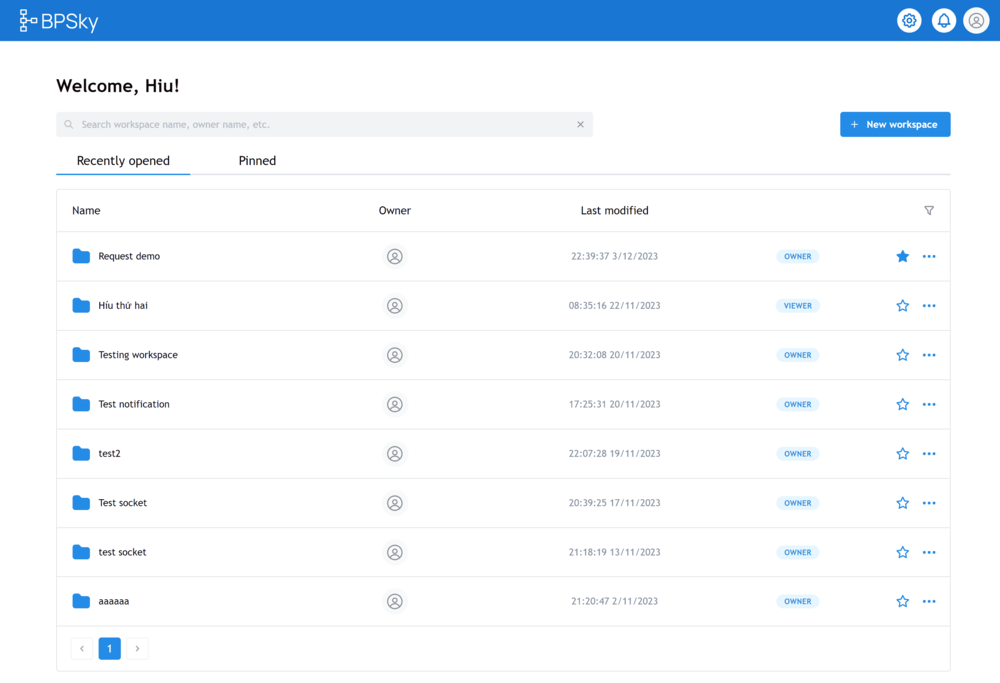
\includegraphics[ width = \linewidth]{Content/Hiện thực hệ thống/documents/Hiện thực giao diện người dùng/images/DefaultHomepage.png}
    \vspace{0.5cm}
    \caption{Giao diện trang default homepage}
    \label{fig: Giao diện trang default homepage}
\end{figure}

Người dùng sau khi đăng nhập hệ thống thành công sẽ được chuyển hướng tới giao diện Default homepage. Tại giao diện mặc định này, hệ thống sẽ hiển thị hai danh sách "Recently opened workspace" - hiển thị danh sách những workspace người dùng tham gia/sở hữu theo thứ tự thời gian mở và "Pinned workspace" - hiển thị danh sách những wokrspace người dùng pin (đánh dấu). Người dùng có thể chọn icon "ba chấm" ở bên phải cùng của mỗi item để mở menu thao tác với mỗi item workspace.

\begin{figure}[H]
    \centering
    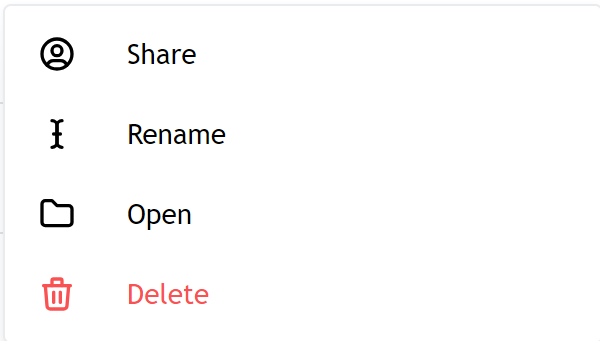
\includegraphics[ width = 0.5\linewidth]{Content/Hiện thực hệ thống/documents/Hiện thực giao diện người dùng/images/DropdownMenu.png}
    \vspace{0.5cm}
    \caption{Dropdown menu}
    \label{fig: Giao diện dropdown menu của mỗi item workspace}
\end{figure}

\begin{figure}[H]
    \centering
    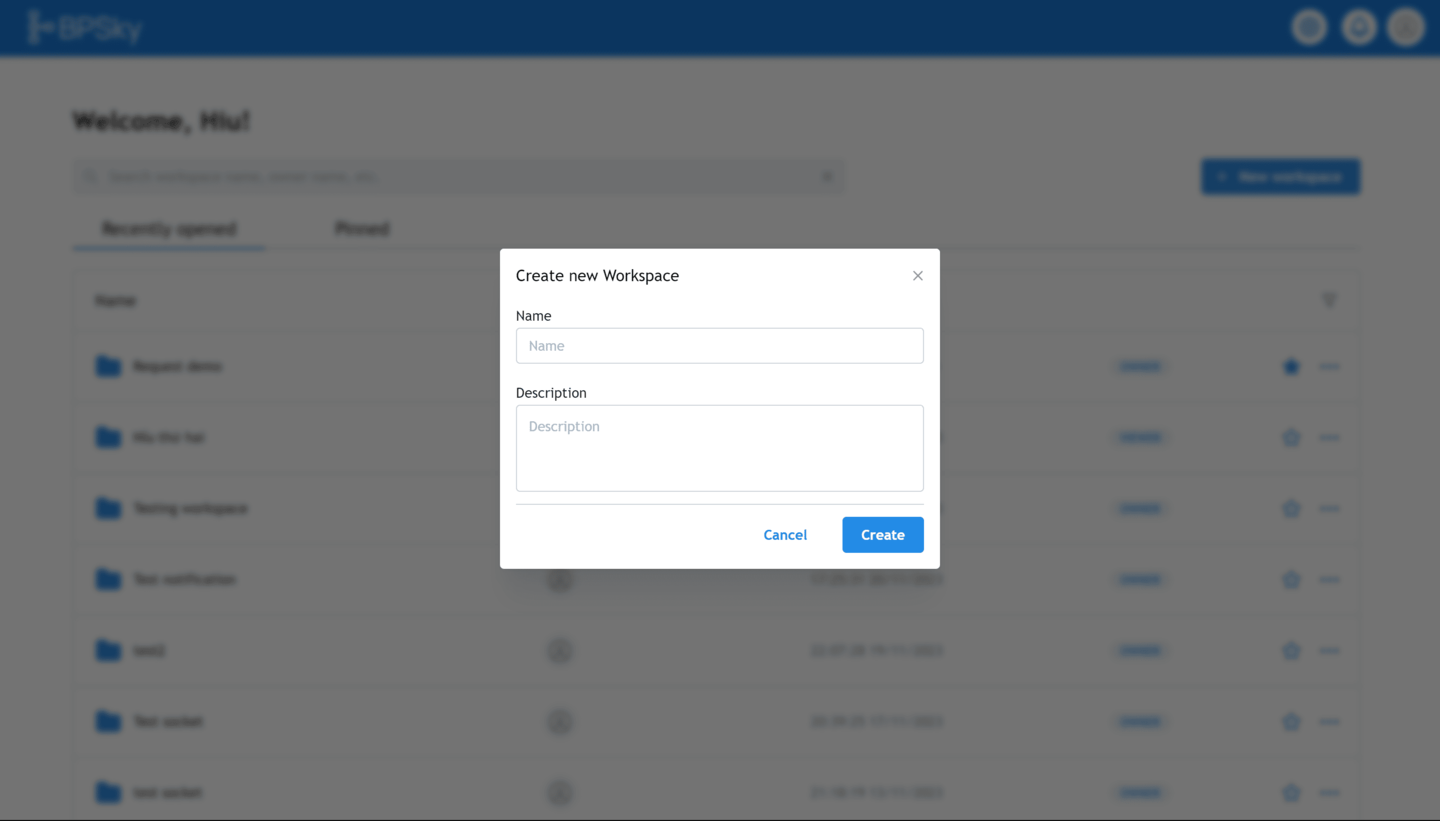
\includegraphics[ width = \linewidth]{Content/Hiện thực hệ thống/documents/Hiện thực giao diện người dùng/images/CreateModal.png}
    \vspace{0.5cm}
    \caption{Giao diện create modal khi người dùng tạo mới workspace}
    \label{fig: Giao diện create modal khi người dùng tạo mới workspace}
\end{figure}

Người dùng có thể tạo mới workspace bằng cách chọn "Create new workspace" từ dropdown menu. Sau khi chọn, hệ thống sẽ hiển thị giao diện create modal như hình \ref{fig: Giao diện create modal khi người dùng tạo mới workspace}. Tại đây, người dùng có thể nhập tên và mô tả cho workspace. Sau khi hoàn tất, người dùng có thể chọn "Create" để tạo mới workspace hoặc "Cancel" để hủy thao tác.

\begin{figure}[H]
    \centering
    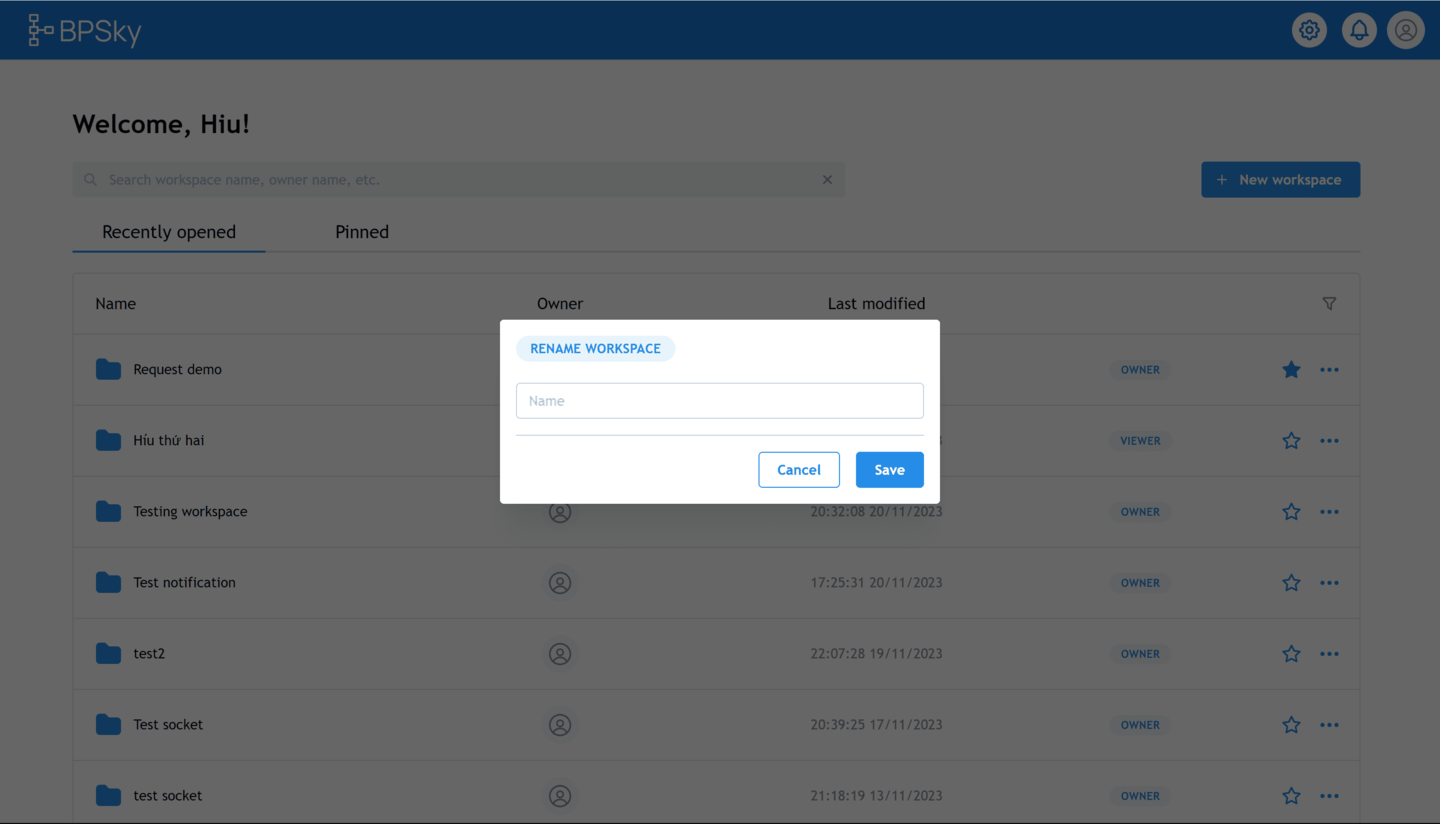
\includegraphics[ width = \linewidth]{Content/Hiện thực hệ thống/documents/Hiện thực giao diện người dùng/images/RenameModal.png}
    \vspace{0.5cm}
    \caption{Giao diện rename modal khi người dùng đổi tên workspace}
    \label{fig: Giao diện rename modal khi người dùng đổi tên workspace}
\end{figure}

Người dùng có thể đổi tên workspace bằng cách chọn "Rename" từ dropdown menu. Sau khi chọn, hệ thống sẽ hiển thị giao diện rename modal như hình \ref{fig: Giao diện rename modal khi người dùng đổi tên workspace}. Tại đây, người dùng có thể nhập tên mới cho workspace. Sau khi hoàn tất, người dùng có thể chọn "Save" để đổi tên workspace hoặc "Cancel" để hủy thao tác.

\begin{figure}[H]
    \centering
    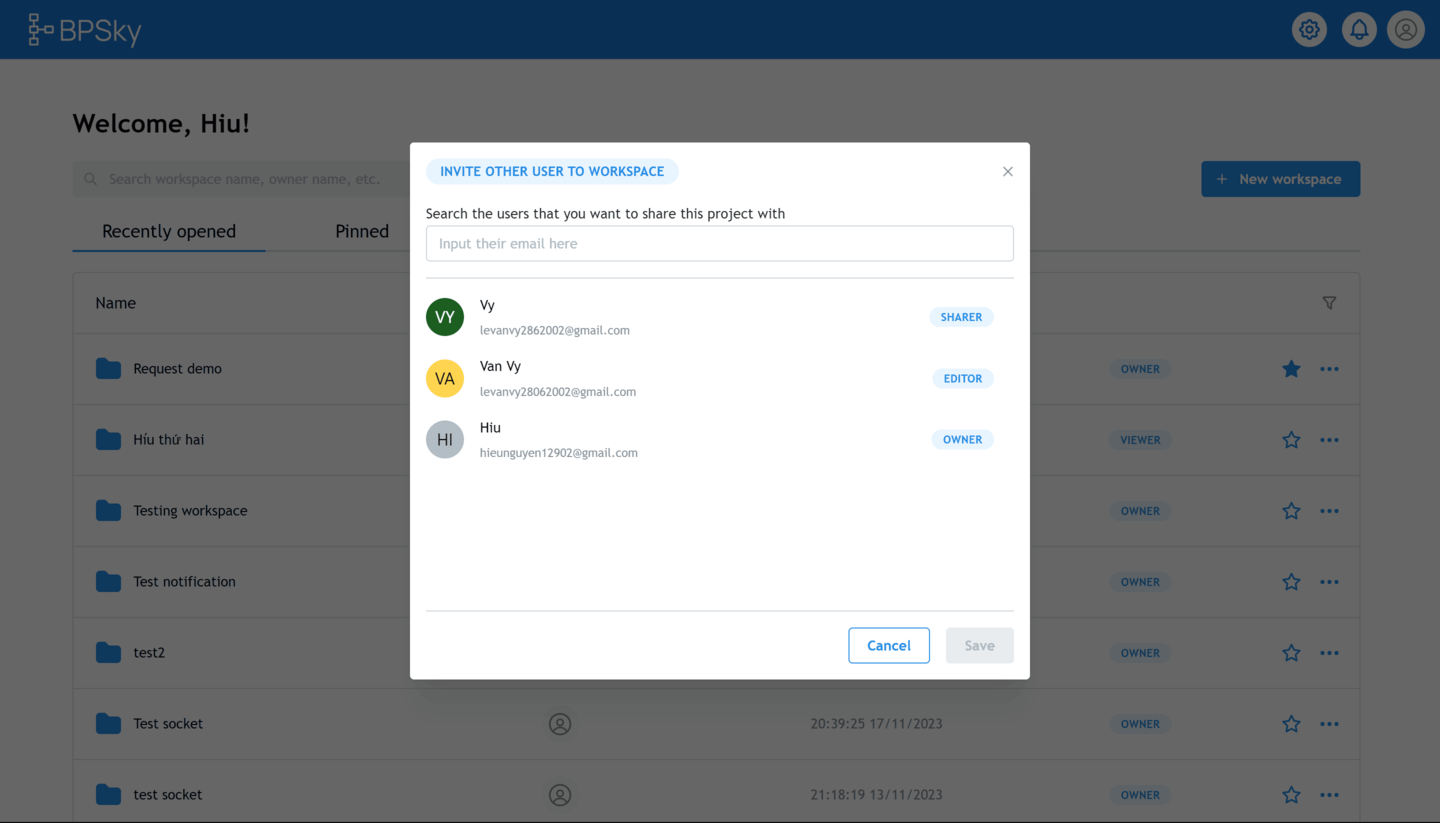
\includegraphics[ width = \linewidth]{Content/Hiện thực hệ thống/documents/Hiện thực giao diện người dùng/images/ShareModal.png}
    \vspace{0.5cm}
    \caption{Giao diện share modal khi người dùng muốn mời/gửi yêu cầu mời người dùng khác vào workspace}
    \label{fig: Giao diện share modal khi người dùng muốn mời/gửi yêu cầu mời người dùng khác vào workspace}
\end{figure}

Người dùng có thể mời người dùng khác vào workspace bằng cách chọn "Share" từ dropdown menu. Sau khi chọn, hệ thống sẽ hiển thị giao diện share modal như hình \ref{fig: Giao diện share modal khi người dùng muốn mời/gửi yêu cầu mời người dùng khác vào workspace}. Tại đây, người dùng có thể nhập tên người dùng mà mình muốn mời vào workspace, sau đó chọn quyền hạn của người được mời vào - quyền hạn của người này không được phép cao hơn người gửi lời mời (owner > editor > sharer > viewer). Sau khi hoàn tất, người dùng có thể chọn "Share" để mời người dùng vào workspace hoặc "Cancel" để hủy thao tác.

\begin{figure}[H]
    \centering
    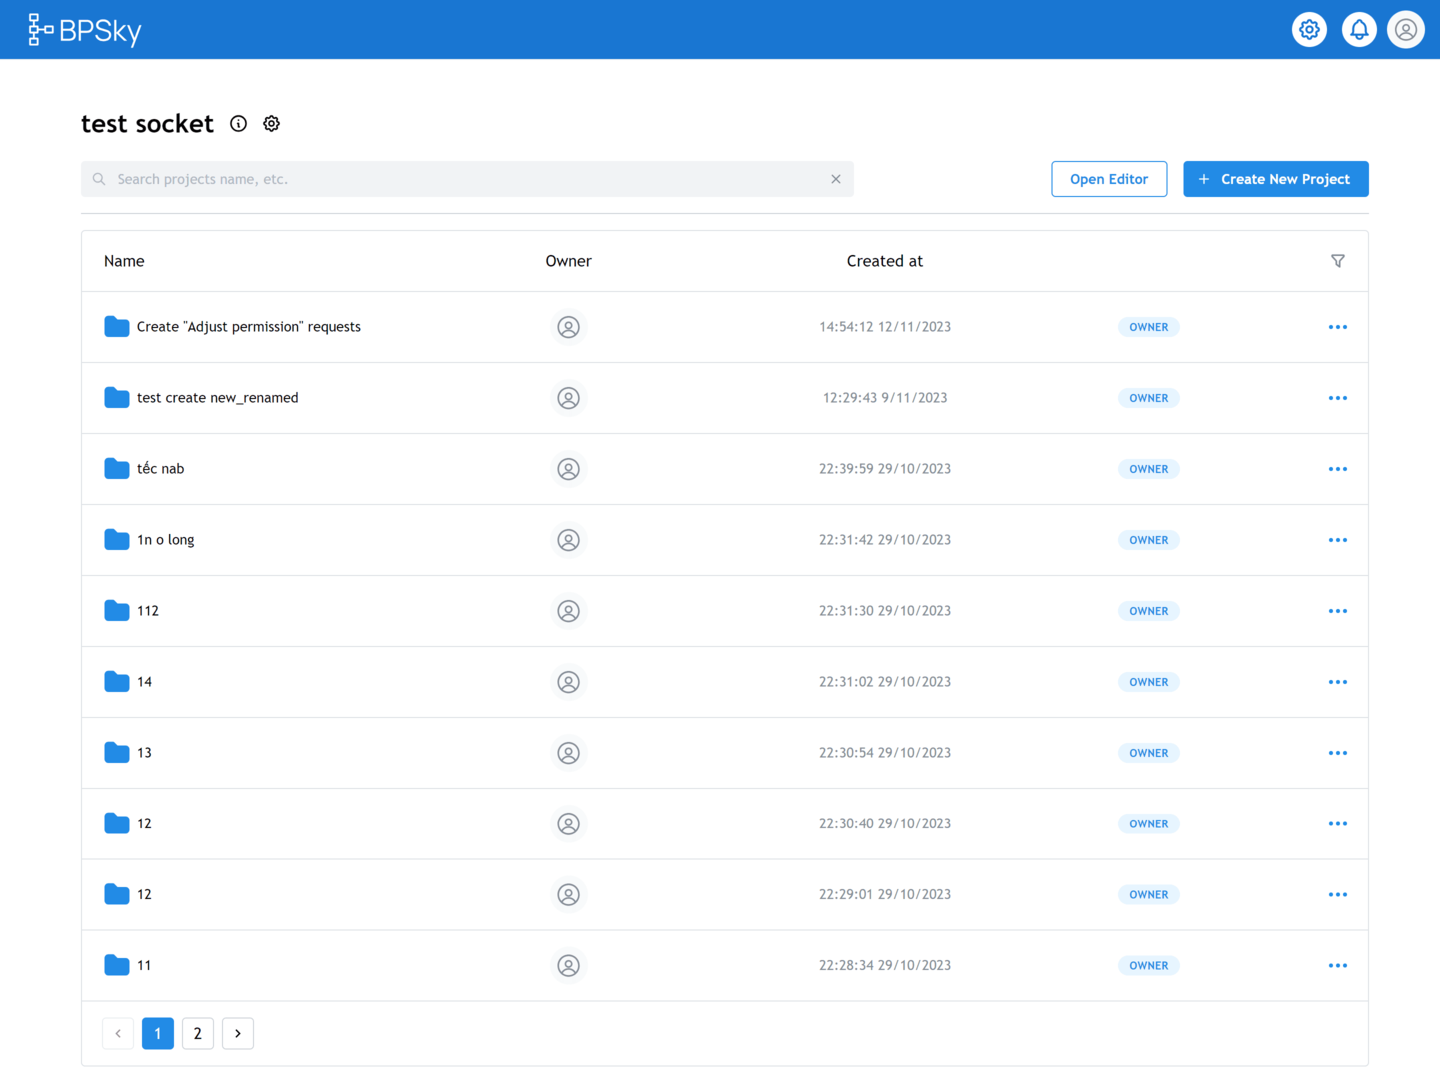
\includegraphics[ width = \linewidth]{Content/Hiện thực hệ thống/documents/Hiện thực giao diện người dùng/images/WorkspaceDetailPage.png}
    \vspace{0.5cm}
    \caption{Giao diện trang Workspace detail}
    \label{fig: Giao diện trang Workspace detail}
\end{figure}

Người dùng có thể truy cập vào trang Workspace detail bằng cách chọn vào tên của workspace từ danh sách các workspace mà người dùng đang tham gia/sở hữu. Tại đây, người dùng có thể xem danh sách những project có trong workspace. Tương tự với danh sách workspace, mỗi item project cũng sẽ có icon "ba chấm" ở phải cùng, người dùng có thể mở dropdown menu để thao tác với project.

\begin{figure}[H]
    \centering
    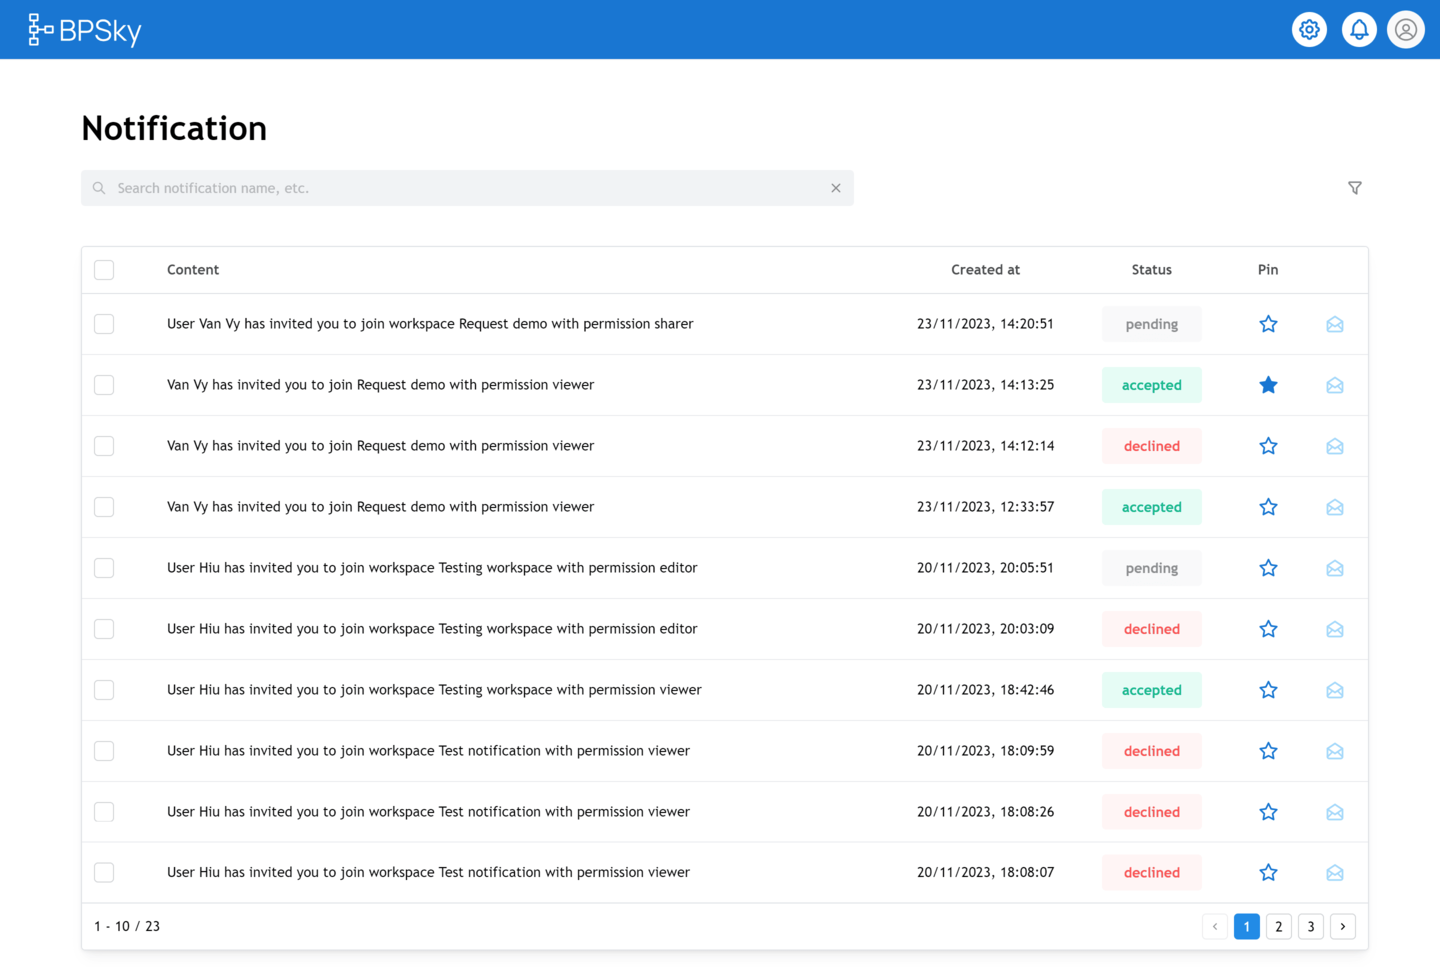
\includegraphics[ width = \linewidth]{Content/Hiện thực hệ thống/documents/Hiện thực giao diện người dùng/images/NotificationPage.png}
    \vspace{0.5cm}
    \caption{Giao diện trang thông báo của người dùng}
    \label{fig: Giao diện trang thông báo của người dùng}
\end{figure}

Người dùng có thể truy cập vào trang thông báo bằng cách chọn icon hình chuông ở phía trên thanh điều hướng. Tại đây, người dùng có thể xem danh sách những thông báo mà hệ thống gửi tới người dùng. Mỗi item thông báo sẽ tùy thuộc vào loại thông báo tương ứng mà hiển thị trạng thái khác nhau (bao gồm "Approved" - chấp nhận, "Declined" - từ chối, "Pending" - đang chờ phản hồi). Người dùng có thể đánh dấu thông báo quan trọng bằng cách nhấn vào icon ngôi sao ở mỗi item thông báo, thông báo quan trọng có thể được lọc thông qua công cụ filter.

\begin{figure}[H]
    \centering
    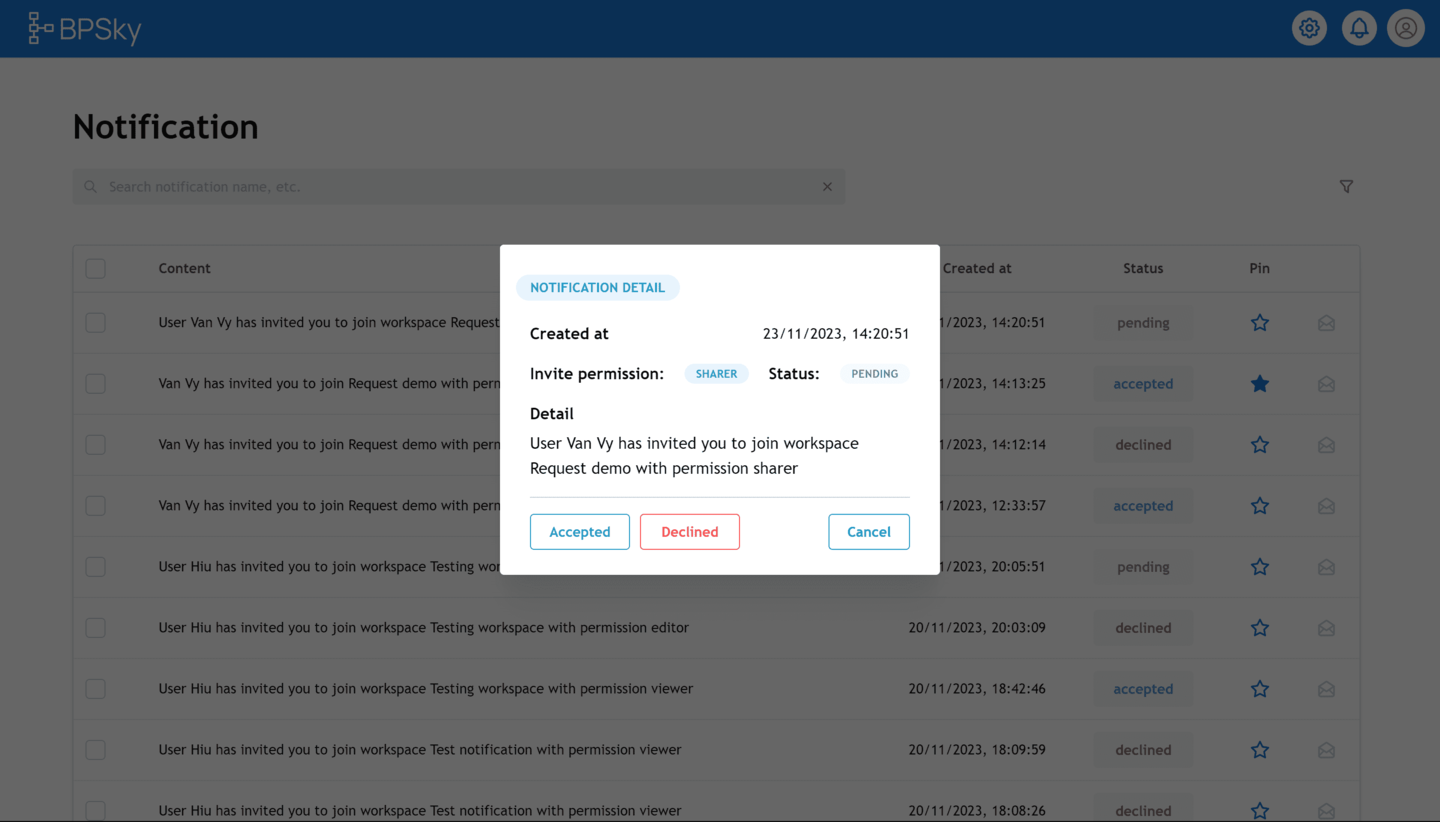
\includegraphics[ width = \linewidth]{Content/Hiện thực hệ thống/documents/Hiện thực giao diện người dùng/images/NotificationDetailModal.png}
    \vspace{0.5cm}
    \caption{Giao diện modal hiển thị thông tin chi tiết của thông báo}
    \label{fig: Giao diện modal hiển thị thông tin chi tiết của thông báo}
\end{figure}

Người dùng có thể xem thông tin chi tiết của mỗi thông báo bằng cách nhấn vào item thông báo tương ứng. Hệ thống sẽ hiển thị giao diện modal như hình \ref{fig: Giao diện modal hiển thị thông tin chi tiết của thông báo}. Tại đây, người dùng có thể xem thông tin chi tiết của thông báo, tùy thuộc vào loại thông báo mà người dùng sẽ có thể tương tác "Approve" - chấp nhận hoặc "Decline" từ chối lời mời được đính kèm trong thông báo. Nếu người dùng muốn đóng modal, người dùng có thể nhấn vào nút "Cancel".

\begin{figure}[H]
    \centering
    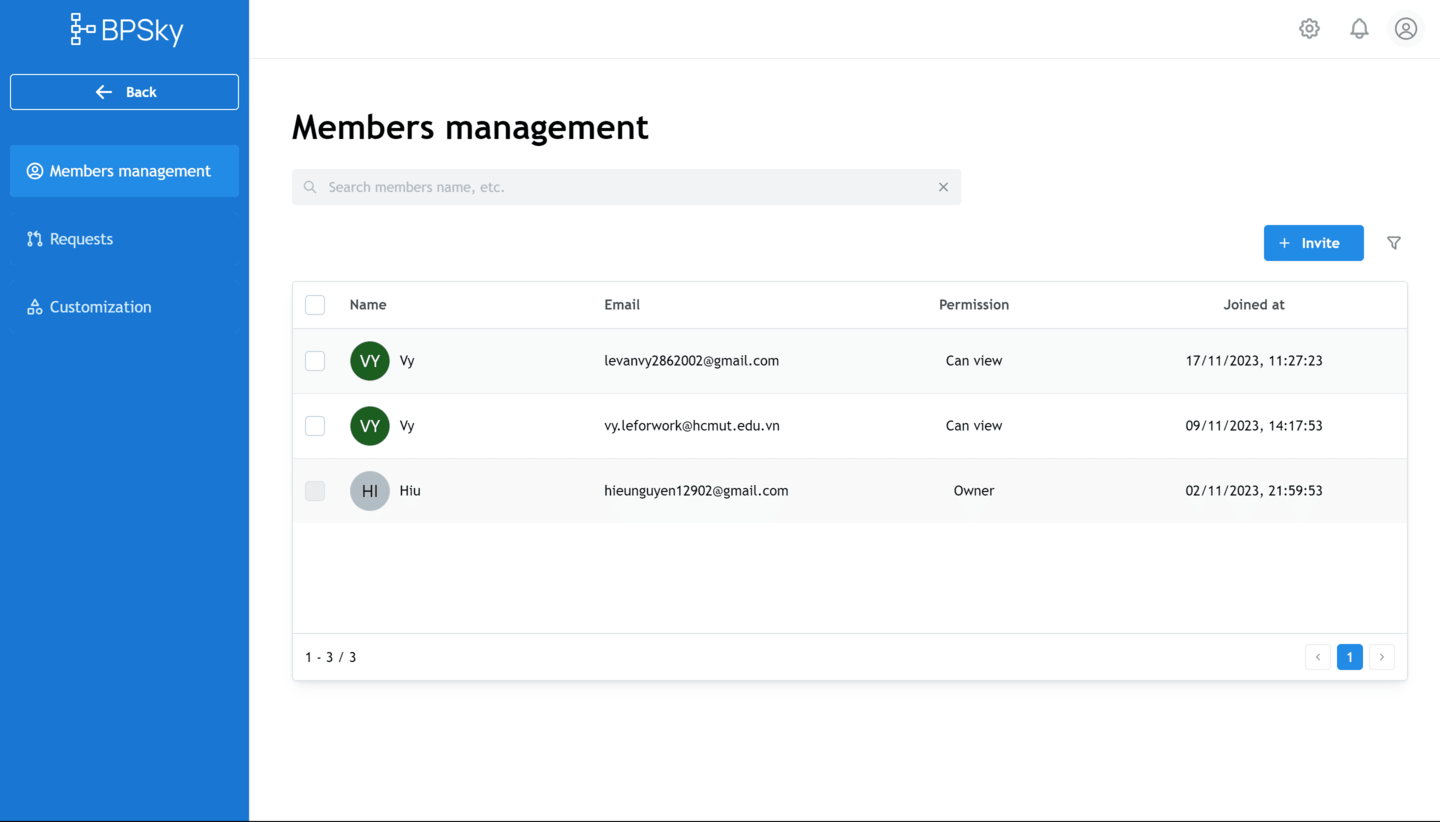
\includegraphics[ width = \linewidth]{Content/Hiện thực hệ thống/documents/Hiện thực giao diện người dùng/images/MembersManagementPage.png}
    \vspace{0.5cm}
    \caption{Giao diện trang quản lý thành viên trong Workspace}
    \label{fig: Giao diện trang quản lý thành viên trong Workspace}
\end{figure}

Nếu người dùng là người sở hữu workspace (workspace owner) thì có thể chọn icon bánh răng bên cạnh tên của workspace tại trang Workspace Detail để điều hướng tới giao diện quản lý workpsace. Người dùng sẽ được điều hướng mặc định tới trang quản lý thành viên trong workspace. Hệ thống sẽ hiển thị danh sách những thành viên có trong workspace cùng với quyền hạn và thời gian tham gia workspace của họ, chúng ta có thể lọc người dùng theo vai trò trong hệ thống. Nếu người sở hữu workspace muốn mời thêm thành viên trong hệ thống vào workspace thì có thể chọn nút "Invite", hệ thống sẽ mở Share modal - Share modal này sẽ gửi lời mời trực tiếp đến người dùng thông qua hòm thông báo.

\begin{figure}[H]
    \centering
    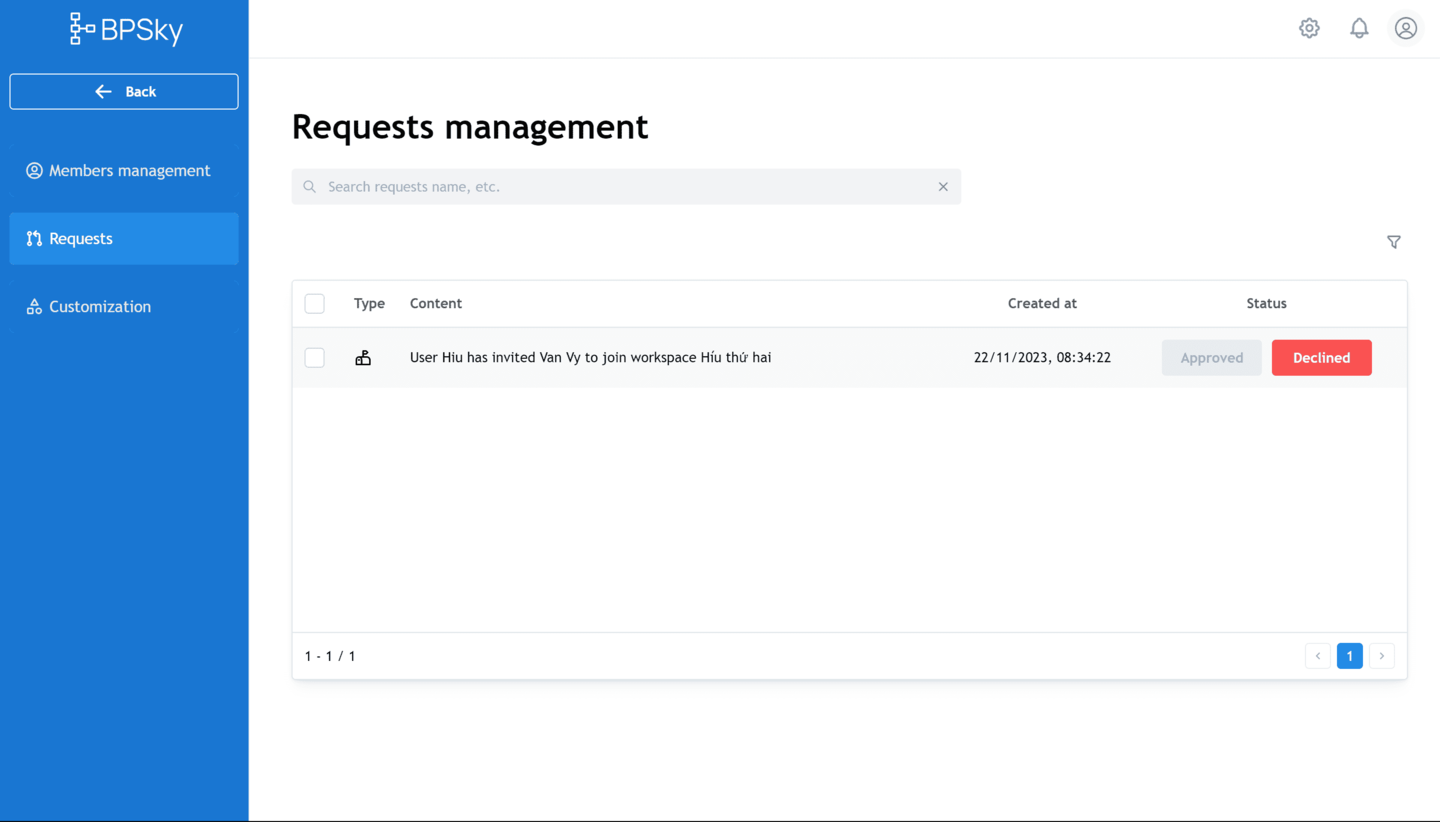
\includegraphics[ width = \linewidth]{Content/Hiện thực hệ thống/documents/Hiện thực giao diện người dùng/images/RequestsManagementPage.png}
    \vspace{0.5cm}
    \caption{Giao diện trang quản lý yêu cầu từ thành viên trong workspace}
    \label{fig: Giao diện trang quản lý yêu cầu từ thành viên trong workspace}
\end{figure}

\begin{figure}[H]
    \centering
    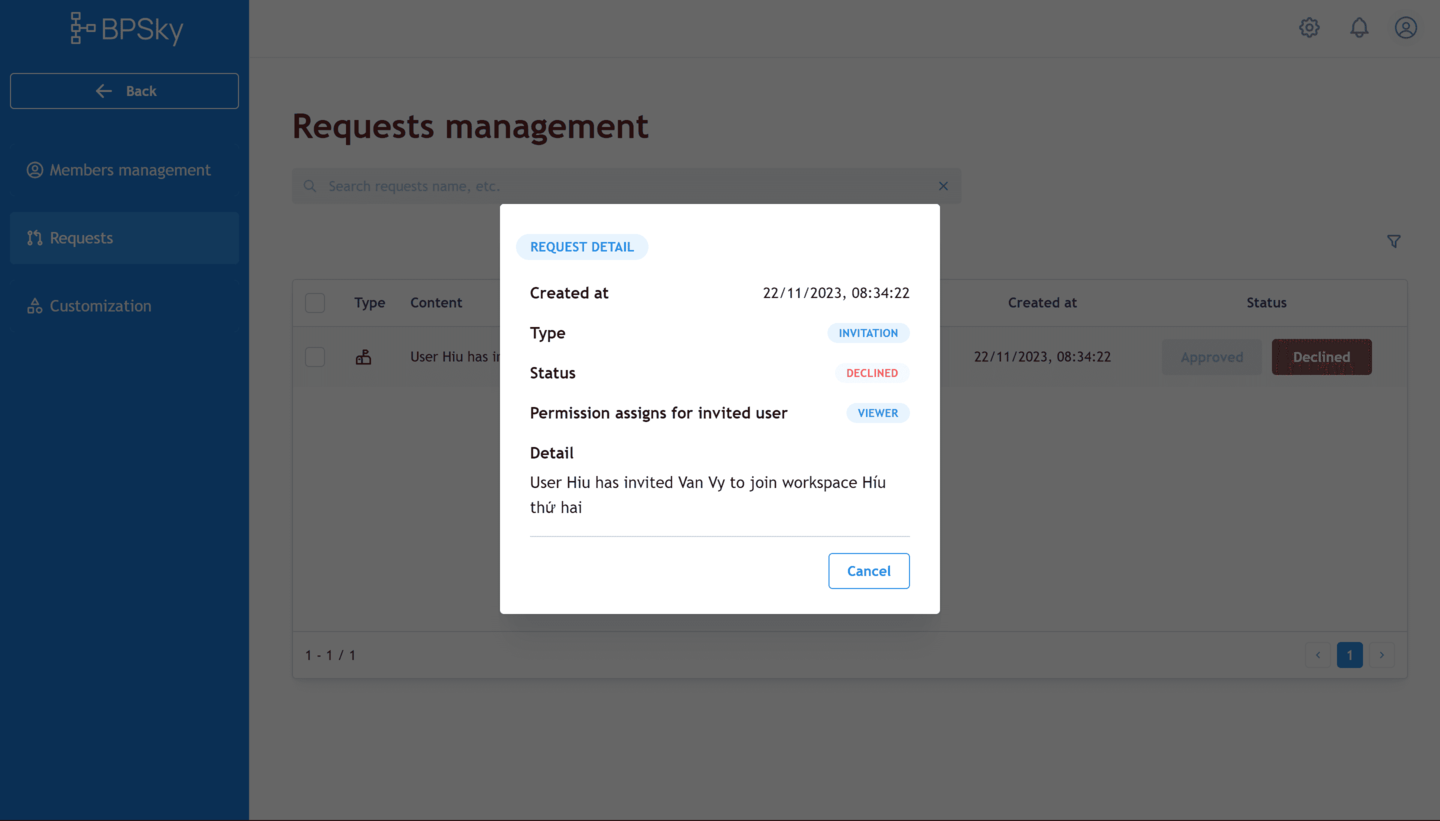
\includegraphics[ width = \linewidth]{Content/Hiện thực hệ thống/documents/Hiện thực giao diện người dùng/images/RequestDetailModal.png}
    \vspace{0.5cm}
    \caption{Giao diện modal hiển thị thông tin chi tiết của yêu cầu}
    \label{fig: Giao diện modal hiển thị thông tin chi tiết của yêu cầu}
\end{figure}

Khi người dùng chọn "Request management" ở thanh sidebar thì hệ thống sẽ chuyển hướng người dùng tới trang quản lý yêu cầu của workspace. Tại đây, hệ thống sẽ hiển thị danh sách những yêu cầu được gửi từ phía thành viên bên trong workspace. Các yêu cầu từ phía thành viên sẽ được phân thành 2 loại: Yêu cầu điều chỉnh vai trò trong workspace và Yêu cầu mời thành viên bên ngoài vào workspace. Người dùng có thể chọn "Approve" hoặc "Decline" để phản hồi yêu cầu tương ứng. Nếu người dùng muốn xem thông tin chi tiết của yêu cầu, người dùng có thể nhấn vào item yêu cầu tương ứng, hệ thống sẽ hiển thị modal như hình \ref{fig: Giao diện modal hiển thị thông tin chi tiết của yêu cầu}.
